%++++++++++++++++++++++++++++++++++++++++
\documentclass[article, 12pt]{article}
\usepackage{float}
\usepackage{setspace}
\usepackage{tabu} % extra features for tabular environment
\usepackage{amsmath}  % improve math presentation
\usepackage{graphicx} % takes care of graphic including machinery
\usepackage[margin=1in]{geometry} % decreases margins
\usepackage{cite} % takes care of citations
\usepackage[final]{hyperref} % adds hyper links inside the generated pdf file
\usepackage{tikz}
\usepackage{caption} 
\usepackage{fancyhdr}
\usepackage{amssymb} % symbols like /therefore
\usepackage{amsthm} % proofs
\usepackage{enumerate} % lettered lists
\usepackage{mathtools} % macros 
\usepackage{tkz-graph}
\usepackage{tikz-layers}
\usepackage[colour, all, curve, arc, frame]{xy} % for diagrams
\usetikzlibrary{scopes}
% \usepackage{xcolor} \pagecolor[rgb]{0.12549019607,0.1294117647,0.13725490196} \color[rgb]{0.82352941176,0.76862745098,0.62745098039} % dark theme
\theoremstyle{definition}
\newtheorem{example}{Example}[subsubsection]
\newtheorem*{remark}{Remark}
\newtheorem{theorem}{Theorem}[subsubsection]
\newtheorem{definition}{Definition}[subsubsection]
\newtheorem{corollary}{Corollary}[subsubsection]
\hypersetup{
	colorlinks=false,      % false: boxed links; true: colored links
	linkcolor=blue,        % color of internal links
	citecolor=blue,        % color of links to bibliography
	filecolor=magenta,     % color of file links
	urlcolor=blue         
}
\usepackage{physics}
\usepackage{siunitx}
\usepackage{tikz,pgfplots}
\usepackage[outline]{contour} % glow around text
\usetikzlibrary{calc}
\usetikzlibrary{angles,quotes} % for pic
\usetikzlibrary{arrows.meta}
\usetikzlibrary{automata}
\usetikzlibrary{arrows.meta, automata, positioning, quotes}
\tikzset{>=latex} % for LaTeX arrow head
\contourlength{1.2pt}

\colorlet{xcol}{blue!70!black}
\colorlet{vcol}{green!60!black}
\colorlet{myred}{red!70!black}
\colorlet{myblue}{blue!70!black}
\colorlet{mygreen}{green!70!black}
\colorlet{mydarkred}{myred!70!black}
\colorlet{mydarkblue}{myblue!60!black}
\colorlet{mydarkgreen}{mygreen!60!black}
\colorlet{acol}{red!50!blue!80!black!80}
\tikzstyle{CM}=[red!40!black,fill=red!80!black!80]
\tikzstyle{xline}=[xcol,thick,smooth]
\tikzstyle{mass}=[line width=0.6,red!30!black,fill=red!40!black!10,rounded corners=1,
                  top color=red!40!black!20,bottom color=red!40!black!10,shading angle=20]
\tikzstyle{faded mass}=[dashed,line width=0.1,red!30!black!40,fill=red!40!black!10,rounded corners=1,
                        top color=red!40!black!10,bottom color=red!40!black!10,shading angle=20]
\tikzstyle{rope}=[brown!70!black,very thick,line cap=round]
\def\rope#1{ \draw[black,line width=1.4] #1; \draw[rope,line width=1.1] #1; }
\tikzstyle{force}=[->,myred,very thick,line cap=round]
\tikzstyle{velocity}=[->,vcol,very thick,line cap=round]
\tikzstyle{Fproj}=[force,myred!40]
\tikzstyle{myarr}=[-{Latex[length=3,width=2]},thin]
\def\tick#1#2{\draw[thick] (#1)++(#2:0.12) --++ (#2-180:0.24)}
\DeclareMathOperator{\sn}{sn}
\DeclareMathOperator{\cn}{cn}
\DeclareMathOperator{\dn}{dn}
\def\N{80} % number of samples in plots


\usepackage{titling}
\usepackage{nicematrix}
\renewcommand\maketitlehooka{\null\mbox{}\vfill}
\renewcommand\maketitlehookd{\vfill\null}
\usepackage{siunitx} % units
\usepackage{verbatim} 
\newcommand{\courseNumber}{MATH 263}
\newcommand{\courseName}{Discrete Mathematics 2}
\newcommand{\professor}{Dr. Petrescu}
\newcommand{\psetName}{Homework 3}
\newcommand{\dueDate}{Due: March 3, 2023}
\newcommand{\name}{Denny Cao}
\pagestyle{fancy}
\fancyhf{}% clears all header and footer fields
\fancyfoot[C]{--~\thepage~--}
\renewcommand*{\headrulewidth}{0.4pt}
\renewcommand*{\footrulewidth}{0pt}
\lhead{\name}
\chead{\courseNumber: \courseName}
\rhead{\professor}
\newcounter{questionNumber}

% Theorems for problem and answer
\newtheorem{question}{Question}
\newtheorem{answer}{Answer}

\fancypagestyle{plain}{%
  \fancyhf{}% clears all header and footer fields
  \fancyfoot[C]{--~\thepage~--}%
  \renewcommand*{\headrulewidth}{0pt}%
  \renewcommand*{\footrulewidth}{0pt}%
}

% Shortcuts
\DeclarePairedDelimiter\ceil{\lceil}{\rceil} % ceil function
\DeclarePairedDelimiter\floor{\lfloor}{\rfloor} % floor function

\DeclarePairedDelimiter\paren{(}{)} % parenthesis

\newcommand{\df}{\displaystyle\frac} % displaystyle fraction
\newcommand{\qeq}{\overset{?}{=}} % questionable equality

\newcommand{\Mod}[1]{\;\mathrm{mod}\; #1} % modulo operator

\newcommand{\comp}{\circ} % composition

% Sets
\DeclarePairedDelimiter\set{\{}{\}}
\newcommand{\unite}{\cup}
\newcommand{\inter}{\cap}

\newcommand{\reals}{\mathbb{R}} % real numbers: textbook is Z^+ and 0
\newcommand{\ints}{\mathbb{Z}}
\newcommand{\nats}{\mathbb{N}}
\newcommand{\tots}{\mathbb{Q}}

\newcommand{\degree}{^\circ}

% Counting
\newcommand\perm[2][^n]{\prescript{#1\mkern-2.5mu}{}P_{#2}}
\newcommand\comb[2][^n]{\prescript{#1\mkern-0.5mu}{}C_{#2}}

% Relations
\newcommand{\rel}{\mathcal{R}} % relation

\setlength\parindent{0pt}

% Directed Graphs
\usetikzlibrary{arrows}
\tikzset{vertex/.style = {shape=circle,draw,minimum size=2em}}
\tikzset{svertex/.style = {shape=circle,draw,minimum size=.05em,font=\tiny}}
\tikzset{edge/.style = {->,> = latex'}}
\tikzset{dedge/.style = {-> = latex'}}

% Contradiction
\newcommand\contradiction{\mathbin{\mathpalette\xhash\relax}}
\newcommand{\xhash}[2]{\ooalign{%
  $#1\xxhash{#1}{-45}$\cr
  $#1\xxhash{#1}{45}$\cr
  }%
}
\newcommand{\xxhash}[2]{\rotatebox[origin=c]{#2}{$#1\parallel$}}

%++++++++++++++++++++++++++++++++++++++++
% title stuff

\makeatletter
\renewcommand{\maketitle}{\bgroup\setlength{\parindent}{0pt}
    \begin{flushleft}
        \textbf{\@title} \\ \vskip0.2cm
        \begingroup
            \fontsize{14pt}{12pt}\selectfont
            \courseNumber: \courseName 
            \vskip0.3cm 
            \professor
        \endgroup \vskip0.3cm
        \@date \hfill\rlap{}\bf{\name} \\ \vskip0.1cm
        \hrulefill
    \end{flushleft}\egroup 
}
\makeatother

\title{\Huge\bf{\psetName}}
\author{\name}
\date{\dueDate}

\author{\name}
\date{\dueDate}

\begin{document}
    \maketitle
    \thispagestyle{empty}

    % Question 1
    \begin{question}
        Solve the traveling salesperson problem for this graph by finding the total weight of all Hamilton circuits and determining a circuit with minimum total weight.  
        \begin{figure}[H]
            \hfil
            \xygraph{ !{<0cm,0cm>;<2cm,0cm>:<0cm,2cm>::} !~-{@{-}@[|(3)]@[red]}!{(0,0) }*+[blue]{\bullet_{a}}="a" !{(1,1) }*+[blue]{\bullet_{b}}="b" !{(2,1) }*+[blue]{\bullet_{c}}="c" !{(1,-1)}*+[blue]{\bullet_{d}}="d"  "a"-"c"_(0.7){7}  "a"-"b"^(0.5){3} "a"-"d"_(0.3){4} "d" -"b" ^(0.4){9}  "b"-"c"^(0.4){6}  "c"-"d"^(0.6){4} }
        \end{figure}
    \end{question}

    % Answer 1
    \begin{answer}
        There are 3 Hamilton circuits. 

        $H_1 = a,b,c,d,a$ with total weight $3 + 6 + 4 + 4 = 17$.
        
        $H_2 = a,c,b,d,a$ with total weight $7+6+9+4=26$.
        
        $H_3 = a,c,d,b,a$ with total weight $7+4+9+3=23$.

        The circuit with minimum total weight is $H_1,$ or $a,b,c,d,a$ with total weight 17.
    \end{answer}
    % Question 2
    \begin{question}
        Try to draw the given  graph without any crossings.  If it is not possible explain why.
        \begin{figure}[H]
                \hfil
                \xygraph{ !{<0cm,0cm>;<2cm,0cm>:<0cm,2cm>::}!~-{@{-}@[|(2.5)]@[blue]} !{(2,2) }*+{\bullet_{a}}="a" !{(1,1) }*+{\bullet_{b}}="b" !{(2,0) }*+{\bullet_{e}}="e" !{(3,1)}*+{\bullet_{c}}="c"!{(0,0)}*+{\bullet_{d}}="d" !{(4,0)}*+{\bullet_{f}}="f"  "a"-"b" "a"-"c"  "a"-"e" "b"-"d" "f"-"b" "d"- "c"   "d"-"e"  "f"-"e" "f"-"c"  }
        \end{figure}
    \end{question}
    
    % Answer 2
    \begin{answer}
        It is not possible to draw the graph which we will denote $G$ without any crossings. 
        \begin{proof}
            We will prove this by showing that the graph is homeomorphic to $K_{3,3}$. Let $K_{3,3}$ be drawn as follows:
            \begin{figure}[H]
                \hfil
                \xygraph{ !{<0cm,0cm>;<2cm,0cm>:<0cm,2cm>::}!~-{@{-}@[|(2.5)]@[blue]} !{(0,2) }*+{\bullet_{a'}}="a" !{(2,2) }*+{\bullet_{b'}}="b" !{(2,0) }*+{\bullet_{e'}}="e" !{(2,1)}*+{\bullet_{c'}}="c"!{(0,0)}*+{\bullet_{d'}}="d" !{(0,1)}*+{\bullet_{f'}}="f"  "a"-"b" "a"-"c"  "a"-"e" "b"-"d" "f"-"b" "d"- "c"   "d"-"e"  "f"-"e" "f"-"c"  }
            \end{figure}
            Let $V_1$ denote the vertex set of $G$. Let $V_2$ denote the vertex set of $K_{3,3}$. We construct a function $g: V_1 \rightarrow V_2$ by $g(a) = a'$, $g(b) = b'$, $g(c) = c'$, $g(d) = d'$, $g(e) = e'$, and $g(f) = f'$. Let $A_1$ be the adjacency matrix of $G$ and $A_2$ be the adjacency matrix of $K_{3,3}$
            \begin{align*}
                \NiceMatrixOptions{code-for-first-row=\scriptstyle,code-for-last-row=\scriptstyle}
                A_1 &= \begin{bNiceMatrix}[first-row, first-col]
                     & a & b & c & d & e & f \\
                    a & 0 & 1 & 1 & 0 & 1 & 0 \\
                    b & 1 & 0 & 0 & 1 & 0 & 1 \\
                    c & 1 & 0 & 0 & 1 & 0 & 1 \\
                    d & 0 & 1 & 1 & 0 & 1 & 0 \\
                    e & 1 & 0 & 0 & 1 & 0 & 1 \\
                    f & 0 & 1 & 1 & 0 & 1 & 0 
                \end{bNiceMatrix} \quad 
                A_2 = \begin{bNiceMatrix}[first-row, first-col]
                    & a' & b' & c' & d' & e' & f' \\
                   a' & 0 & 1 & 1 & 0 & 1 & 0 \\
                   b' & 1 & 0 & 0 & 1 & 0 & 1 \\
                   c' & 1 & 0 & 0 & 1 & 0 & 1 \\
                   d' & 0 & 1 & 1 & 0 & 1 & 0 \\
                   e' & 1 & 0 & 0 & 1 & 0 & 1 \\
                   f' & 0 & 1 & 1 & 0 & 1 & 0 
               \end{bNiceMatrix} 
            \end{align*}
            As the adjacency matrices of $G$ and $K_{3,3}$ are the same for corresponding vertices, we have that $g$ is a homeomorphism from $G$ to $K_{3,3}$. Thus, $G$ is not planar, meaning that it cannot be drawn without any crossings.
        \end{proof}
    \end{answer}

    % Question 3
    \begin{question}
        An edge coloring of a graph is an assignment of colors to edges so that edges incident with a common vertex are assigned different colors. The edge chromatic number of a graph is the smallest number of colors that can be used in an edge coloring of the graph. The edge chromatic number of a graph G is denoted by $\chi(G)$.  Find the edge chromatic numbers of: \vskip.3cm\hskip1cm a) $C_n$, where  $n \ge 3$.\hskip3.5cm b) $W_n$, where $n \ge 3$.
    \end{question}

    % Answer 3
    \begin{answer}
        
    \end{answer}
    \begin{enumerate}[a)]
        \item $\chi(C_n) = \begin{cases}
            2 & n \text{ is even} \\
            3 & n \text{ is odd}
        \end{cases}$
        \begin{proof}
            Let $E_x$ represent the $x$th edge of $C_n$, where $1 \leq x \leq n-1, x \in \ints$. In $C_n$, an edge $E_c$ share a vertex with $E_{c+1}$ and a different vertex with $E_{c-1}$, and if $c=1$, then $E_c$ shares a vertex with $E_n$ and if $c=n-1$, then $E_c$ shares a vertex with $E_1$. 

            \textit{Case 1:} $n$ is even. In this case, we can color $E_2k$ with one color and $E_{2k-1}$ with another color for all $k \in \ints$ such that $1 \leq k \leq \frac{n}{2}$. Thus, we can color $C_n$ with two colors, as each vertex has an even and odd edge.

            \textit{Case 2:} $n$ is odd. In this case, $E_n$ and $E_1$ share a vertex, though $n$ and 1 are both odd. Thus, we can color $E_2k$ with one color and $E_{2k-1}$ with another color for all $k \in \ints$ such that $1 \leq k \leq \frac{n}{2}$. We can then color $E_n$ with a third color. Thus, we can color $C_n$ with three colors.
        \end{proof}
        \item $\chi(W_n) = n$
        \begin{proof}
            The center vertex of $W_n$ has degree $n$, and therefore there must be at least $n$ colors to color the edges of $W_n$. The outer vertices of $W_n$ have degree 3, which is less than or equal to $n$ and thus $n$ colors is enough to color the edges of $W_n$.
        \end{proof}
    \end{enumerate}
    % Question 4
    \begin{question}
        Find the edge chromatic number of $K_n$ when n is a positive integer.
    \end{question}
    
    % Answer 4
    \begin{answer}
        \begin{equation*}
            \chi(K_n) = \begin{cases}
                n - 1 & n \text{ is even} \\
                n & n \text{ is odd}
            \end{cases}
        \end{equation*}
    \end{answer}
    \begin{proof} As each vertex is connected with $n-1$ other vertices, there are a total of $n(n-1)/2$ edges.
        \\[12pt]
        \textit{Case 1:} $n$ is even. A separate color can be assigned to $\frac{n}{2}$ vertices, where none share a vertex. Thus, as $\frac{n(n-1)}{2} / \frac{n}{2} = n-1$, we can color $K_n$ with $n-1$ colors.
        \\[12pt]
        \textit{Case 2}: $n$ is odd. $\frac{n-1}{2}$ edges can be assigned to each color, where none share a vertex. Thus, as $\frac{n(n-1)}{2} / \frac{n-1}{2} = n$, we can color $K_n$ with $n$ colors.
    \end{proof}
    % Question 5
    \begin{question}
        Show that if $G$ is a bipartite simple graph with $v$ vertices and $e$ edges, then $e \leq \frac{v^2}4$.
    \end{question}

    % Answer 5
    \begin{answer}
        \begin{proof}
            Let $V$ be the vertex set of $G$ and $E$ be the edge set of $G$. As $G$ is bipartite, we can partition $V$ into two sets $V_1$ and $V_2$, where $\forall a,b \in V_1, \forall c,d \in V_2 ((a,b) \not\in E \land (c,d) \not\in E)$. The maximum amount of edges then, will be when all vertices in $V_1$ are connected to all vertices in $V_2$. This will give us $|V_1| \cdot |V_2|$ edges. The total vertices, $v$, is equal to $|V_1| + |V_2|$. We will maximize $|V_1| \cdot |V_2|$ with the constraint that $|V_1| + |V_2| = v$. Let $f(|V_1|,|V_2|) = |V_1| \cdot |V_2|$, the function we are optimizing, and $g(|V_1|,|V_2|) = |V_1| + |V_2| - v$, our constraint. We can then write the Lagrangian function as:
            \begin{align*}
                F(|V_1|,|V_2|,\lambda) &= f(|V_1|,|V_2|) + \lambda g(|V_1|,|V_2|) \\
                               &= |V_1| \cdot |V_2| + \lambda(|V_1| + |V_2| - v) \\
                \grad F        = \begin{pmatrix}
                    \frac{\partial F}{\partial |V_1|} \\
                    \frac{\partial F}{\partial |V_2|} \\
                    \frac{\partial F}{\partial \lambda}
                \end{pmatrix} 
                &= \begin{pmatrix}
                    |V_2| + \lambda \\
                    |V_1| + \lambda \\
                    |V_1| + |V_2| - v
                \end{pmatrix} = \begin{pmatrix}
                    0 \\ 
                    0 \\ 
                    0
                \end{pmatrix}
            \end{align*}
            From this, $\lambda = -|V_1| \land \lambda = -|V_2| \to |V_1| = |V_2|$. It follows that $|V_1| + |V_1| - v \to |V_1| = \frac{v}{2}$. As $|V_1| = |V_2|$, $|V_2| = \frac{v}{2}$. Therefore, $|V_1| \cdot |V_2| = \frac{v^2}{4}$. This means that the maximum amount of edges is $\frac{v^2}{4}$. Thus, $e \leq \frac{v^2}{4}$.
        \end{proof}
    \end{answer}
    % Question 6
    \begin{question}
        Suppose that you have a three-gallon jug and a five-gallon jug. You may fill either jug with water, you may empty either jug, and you may transfer water from either jug into the other jug. Use a path in a directed graph to show that you can end up with a jug containing exactly one gallon. [Hint: Use an ordered pair (a, b) to indicate how much water is in each jug. Represent these ordered pairs by vertices. Add an edge for each allowable operation with the jugs.]
    \end{question}

    % Answer 6 
    \begin{answer} \ 
        \begin{figure}[H]
            \centering
            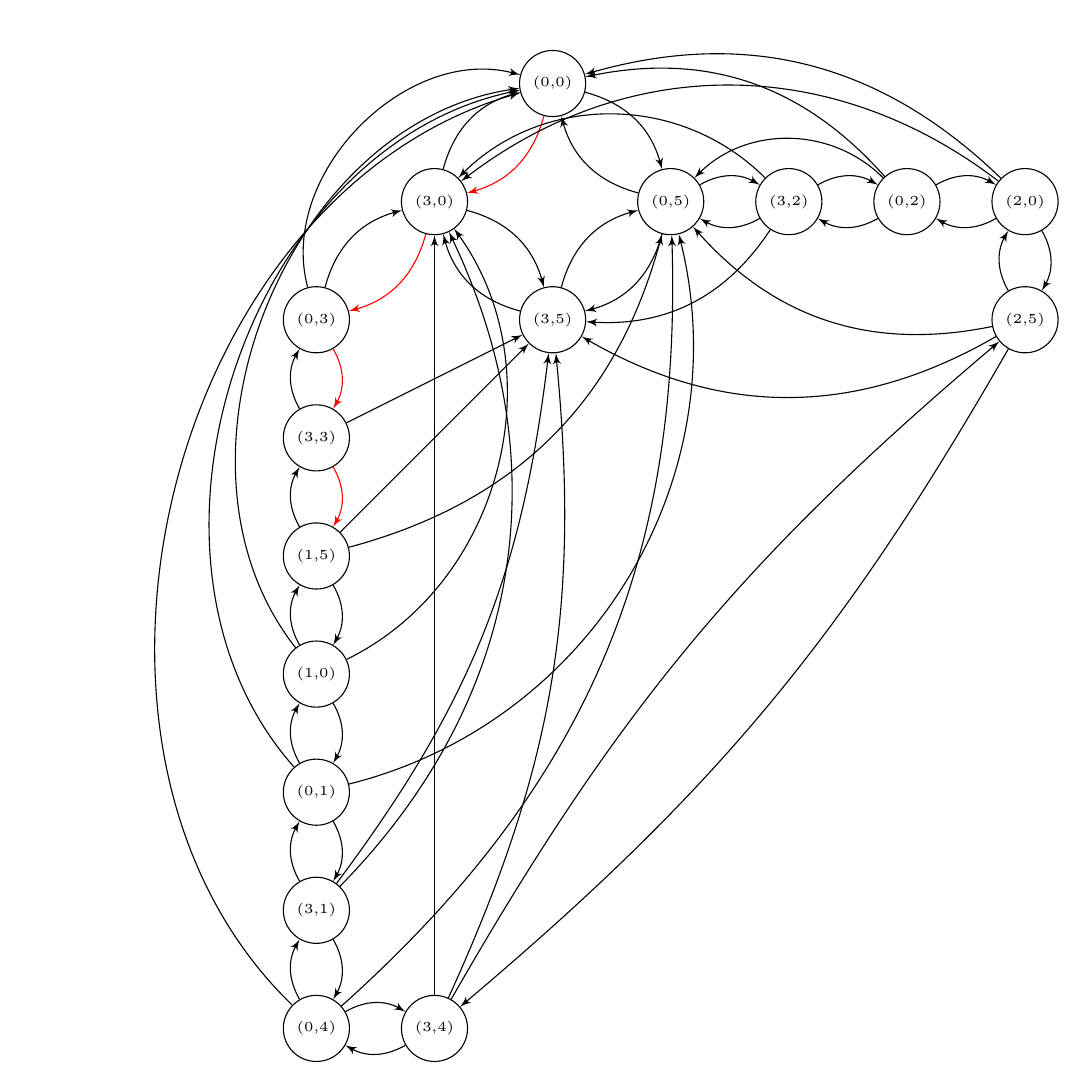
\begin{tikzpicture}[scale=0.75]
                \node[svertex] (00) at (0,0) {(0,0)}; 
                \node[svertex] (30) at (-2,-2) {(3,0)};
                \draw[edge, red] (00) to[bend left] (30); 
                \draw[edge] (30) to[bend left] (00); 
                \node[svertex] (05) at (2,-2) {(0,5)};  
                \draw[edge] (00) to[bend left] (05);
                \draw[edge] (05) to[bend left] (00);    
                \node[svertex] (03) at (-4,-4) {(0,3)};
                \draw[edge, red] (30) to[bend left] (03);
                \draw[edge] (03) to[bend left] (30);
                \draw[edge] (03) to[bend left=60] (00);
                \node[svertex] (35) at (0,-4) {(3,5)};
                \draw[edge] (30) to[bend left] (35);
                \draw[edge] (35) to[bend left] (30);
                \draw[edge] (05) to[bend left] (35);
                \draw[edge] (35) to[bend left] (05);
                \node[svertex] (33) at (-4,-6) {(3,3)};
                \draw[edge, red] (03) to[bend left] (33);
                \draw[edge] (33) to[bend left] (03);
                \draw[edge] (33) to (35);
                \node[svertex] (15) at (-4,-8) {(1,5)};
                \draw[edge] (15) to[bend left] (33);
                \draw[edge] (15) to (35);
                \draw[edge,red] (33) to[bend left] (15);
                \draw[edge] (15) to[bend right] (05);
                \node[svertex] (10) at (-4,-10) {(1,0)};
                \draw[edge] (10) to[bend left] (15);
                \draw[edge] (15) to[bend left] (10);
                \draw[edge] (10) to[bend left=60] (00);
                \node[svertex] (01) at (-4,-12) {(0,1)};
                \draw[edge] (01) to[bend left] (10);
                \draw[edge] (10) to[bend left] (01);
                \draw[edge] (10) to[bend right=50] (30);
                \draw[edge] (01) to[bend left=60] (00);
                \draw[edge] (01) to[bend right=45] (05);
                \node[svertex] (31) at (-4,-14) {(3,1)};
                \draw[edge] (31) to[bend left] (01);
                \draw[edge] (01) to[bend left] (31);
                \draw[edge] (31) to[bend right=15] (35);
                \node[svertex] (04) at (-4,-16) {(0,4)};
                \draw[edge] (04) to[bend left] (31);
                \draw[edge] (31) to[bend left] (04);
                \draw[edge] (31) to[bend right=35] (30);
                \draw[edge] (04) to[bend left=60] (00);
                \draw[edge] (04) to[bend right=25] (05);
                \node[svertex] (34) at (-2, -16) {(3,4)};
                \draw[edge] (34) to[bend left] (04);
                \draw[edge] (04) to[bend left] (34);
                \draw[edge] (34) to[bend right=15] (35);
                \draw[edge] (34) to (30);
                \node[svertex] (32) at (4,-2) {(3,2)};
                \draw[edge] (32) to[bend left] (05);
                \draw[edge] (05) to[bend left] (32);
                \draw[edge] (32) to[bend left] (35);
                \node[svertex] (02) at (6,-2) {(0,2)};
                \draw[edge] (02) to[bend left] (32);
                \draw[edge] (32) to[bend left] (02);
                \draw[edge] (32) to[bend right=45] (30);
                \draw[edge] (02) to[bend right] (00);
                \draw[edge] (02) to[bend right=45] (05);
                \node[svertex] (20) at (8,-2) {(2,0)};
                \draw[edge] (20) to[bend left] (02);
                \draw[edge] (02) to[bend left] (20);
                \draw[edge] (20) to[bend right] (00);
                \draw[edge] (20) to[bend right=37.5] (30);   
                \node[svertex] (25) at (8,-4) {(2,5)};
                \draw[edge] (25) to[bend left] (20);
                \draw[edge] (25) to[bend left] (05);
                \draw[edge] (20) to[bend left] (25);
                \draw[edge] (25) to[bend left] (35);     
                \draw[edge] (25) to[bend left=10] (34);
                \draw[edge] (34) to[bend left=10] (25);        
            \end{tikzpicture}
        \end{figure}
        To end up with a jug containing exactly one gallon, we can follow the path 
        \begin{center}
            $(0,0), (3,0), (0,3), (3,3), (1,5)$
        \end{center}
    \end{answer}
    % Question 7
    \begin{question}
        Find the number of paths of length n between any two adjacent vertices in $K_{3,3}$ for the values of $n$ in $\{3, 4, 5, 6\}$
    \end{question}

    % Answer 7
    \begin{answer}
        The adjacency matrix for $K_{3,3}$ is as follows:
        \begin{equation*}
            A = \begin{bmatrix}
                0 & 0 & 0 & 1 & 1 & 1 \\
                0 & 0 & 0 & 1 & 1 & 1 \\
                0 & 0 & 0 & 1 & 1 & 1 \\
                1 & 1 & 1 & 0 & 0 & 0 \\
                1 & 1 & 1 & 0 & 0 & 0 \\
                1 & 1 & 1 & 0 & 0 & 0
            \end{bmatrix}
        \end{equation*}
        We can then find the number of paths of length $n$ between any two adjacent vertices in $K_{3,3}$ by raising the adjacency matrix to the power $n$.
        
        \begin{align*}
            A^3 = \begin{bmatrix}
                0 & 0 & 0 & 9 & 9 & 9 \\
                0 & 0 & 0 & 9 & 9 & 9 \\
                0 & 0 & 0 & 9 & 9 & 9 \\
                9 & 9 & 9 & 0 & 0 & 0 \\
                9 & 9 & 9 & 0 & 0 & 0 \\
                9 & 9 & 9 & 0 & 0 & 0
            \end{bmatrix} &\quad A^4 = \begin{bmatrix}
                27 & 27 & 27 & 0 & 0 & 0 \\
                27 & 27 & 27 & 0 & 0 & 0 \\
                27 & 27 & 27 & 0 & 0 & 0 \\
                0 & 0 & 0 & 27 & 27 & 27 \\
                0 & 0 & 0 & 27 & 27 & 27 \\
                0 & 0 & 0 & 27 & 27 & 27
            \end{bmatrix} \\
            A^5 = \begin{bmatrix}
                0 & 0 & 0 & 81 & 81 & 81 \\
                0 & 0 & 0 & 81 & 81 & 81 \\
                0 & 0 & 0 & 81 & 81 & 81 \\
                81 & 81 & 81 & 0 & 0 & 0 \\
                81 & 81 & 81 & 0 & 0 & 0 \\
                81 & 81 & 81 & 0 & 0 & 0 \\
            \end{bmatrix} &\quad A^6 = \begin{bmatrix}
                243 & 243 & 243 & 0 & 0 & 0 \\
                243 & 243 & 243 & 0 & 0 & 0 \\
                243 & 243 & 243 & 0 & 0 & 0 \\
                0 & 0 & 0 & 243 & 243 & 243 \\
                0 & 0 & 0 & 243 & 243 & 243 \\
                0 & 0 & 0 & 243 & 243 & 243
            \end{bmatrix}
        \end{align*}
        \textbf{There are 9 paths of length 3, 27 paths of length 4, 81 paths of length 5 and 243 paths of length 6 between any two adjacent vertices in $K_{3,3}$.}

    \end{answer}
    % Question 8
    \begin{question}
        Determine whether  ({\em i}) Dirac's theorem can be used to show  the graphs below have a Hamilton circuit, ({\em ii}) whether Ore's theorem can be used and finally ({\em iii}) if the graph has a Hamilton circuit.
        \begin{figure}[H]
            \centering
            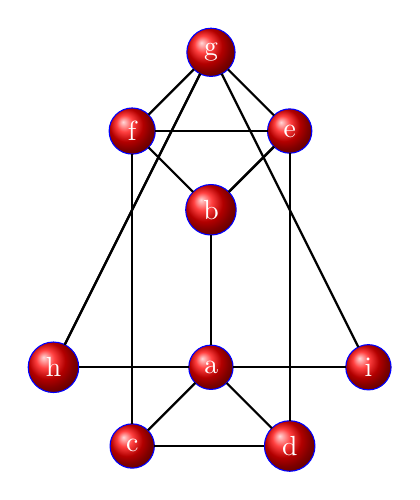
\begin{tikzpicture} \SetGraphUnit{1}\tikzset{VertexStyle/.style ={draw,shape = circle,shading= ball,ball color= red ,minimum size= 16pt,color= blue, text=white}};\coordinate (o) at (0,0);\SO(o){a} \NO(o){b} \SOEA(a){d}\SOWE(a){c}\NOEA(b){e} \NOWE(b){f}\NOEA(f){g}\NOWE(c){h}\NOEA(d){i}\Edges(a,b,f,e,d,a,b,e,g,h,g,i,a)\Edges(d,c,f)\Edges(b,e)\Edges(c,a,h)\Edges(g,f)\end{tikzpicture}
        \end{figure}
    \end{question}

    % Answer 8
    \begin{answer} \ 
        \begin{enumerate}[\em i)]
            \item Dirac's theorem states that an $n$-vertex simple graph with $n \geq 3$ in which each vertex has at least degree $\frac{n}{2}$ has a Hamilton circuit. This theorem cannot be used, as there exists a vertex $g$ with degree 4, which is less than $\frac{9}{2} = 4.5$.
            \item Ore's theorem states that an $n$-vertex simple graph with $n \geq 3$ such that $\deg{u} + \deg{v} \geq n$ for every pair of nonadjacent vertices $u$ and $v$, then the graph has a Hamilton circuit. This theorem cannot be used, as the vertex $g$ has degree 4, and vertex $b$ has degree 3, and $4+3 < 9$.
            \item No, there is no Hamilton circuit in this graph.
        \end{enumerate}    
    \end{answer}

    % Question 9
    \begin{question}
        Find the length of a shortest path between \{({\it x} and {\it z}),( {\it v} and {\it w}), ({\it t} and {\it z})\} in the weighted graph below, using Djikstra algorithm. Show each step.
        \begin{figure}[H]
            \centering
            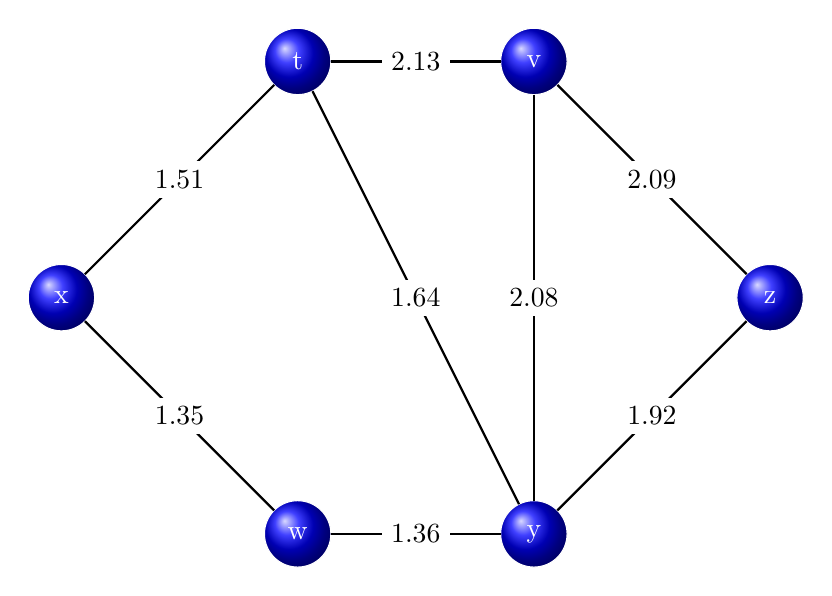
\begin{tikzpicture}\SetGraphUnit{3}\tikzset{VertexStyle/.style ={draw,shape = circle,shading= ball, ball color= blue,minimum size= 24pt, color= white}} \Vertex{x}\NOEA(x){t}\EA(t){v}\SOEA(v){z}\SOWE(z){y}\WE(y){w}\NOWE(w){x}\tikzset{LabelStyle/.style ={fill=white}}\Edge[label=$1.51$](x)(t)\Edge[label=$2.13$](t)(v)\Edge[label=$2.09$](v)(z)\Edge[label=$1.92$](y)(z)\Edge[label=$1.36$](w)(y)\Edge[label=$2.08$](v)(y)\Edge[label=$1.35$](x)(w)\Edge[label=$1.64$](t)(y)\end{tikzpicture}
        \end{figure}
    \end{question}
    
    % Answer 9
    \begin{answer}
        \begin{align*}\begin{array}{cc}
            \text{visited nodes} & \text{current shortest path} \\
            \hline \rule{0pt}{1.2\normalbaselineskip}
            x & 0 \\ 
            x,w & 1.35 \\ 
            x,w,t & 1.51 \\ 
            x,w,t,y & 2.71 \\ 
            x,w,t,y,v & 3.64 \\ 
            x,w,t,y,v,z & 4.63
        \end{array}\end{align*}
        The shortest path between $v$ and $w$ is $v \to y \to w$, length 3.44. 
         \begin{align*}\begin{array}{cc}
            \text{visited nodes} & \text{current shortest path} \\
            \hline \rule{0pt}{1.2\normalbaselineskip}
            v & 0 \\
            v,y & 2.08 \\
            v,y,z & 2.09 \\
            v,y,z,t & 2.13 \\
            v,y,z,t,w & 3.44 \\
            v,y,z,t,w,x & 3.44
        \end{array}\end{align*}
        The shortest path between $t$ and $z$ is $t \to y \to z$, length 3.56. 
         \begin{align*}\begin{array}{cc}
            \text{visited nodes} & \text{current shortest path} \\
            \hline \rule{0pt}{1.2\normalbaselineskip}
            t & 0 \\
            t,x & 1.51 \\
            t,x,y & 1.64 \\
            t,x,y,v & 2.13 \\
            t,x,y,v,w & 2.86 \\
            t,x,y,v,w,z & 3.56
        \end{array}\end{align*}
    \end{answer}

    % Question 10
    \begin{question}
        Prove the following statement: If H is a subgraph of G and G is a planar simple graph, then H is also planar.
    \end{question}

    % Answer 10
    \begin{answer}
        \begin{proof}
            As $G$ is a planar graph, it does not contain a subgraph that is homeomorphic to $K_{3,3}$ or $K_5$ by Kuratowski's Theorem. Since $H$ is a subgraph of $G$, it also does not contain a subgraph that is homeomorphic to $K_{3,3}$ or $K_5$. Thus, $H$ is also planar.
        \end{proof}
    \end{answer}
    % Quesion 11
    \begin{question}
        Find the  chromatic number, $\chi(G)$, of the graph below  and decide whether or not the graph is planar. Justify your answer.  
        \begin{figure}[H]
        \hfil
            \xygraph{ !{<0cm,0cm>;<0cm,2cm>:<-2cm,0cm>::} !{(0,0);a(0)**{}?(1.0)}*{\bullet}="a1" !{(0,0);a(72)**{}?(1.0)}*{\bullet}="a2" !{(0,0);a(144)**{}?(1.0)}*{\bullet}="a3" !{(0,0);a(216)**{}?(1.0)}*{\bullet}="a4" !{(0,0);a(288)**{}?(1.0)}*{\bullet}="a5" !{(0,0);a(0)**{}?(1.8)}*{\bullet}="b1" !{(0,0);a(72)**{}?(1.8)}*{\bullet}="b2" !{(0,0);a(144)**{}?(1.8)}*{\bullet}="b3" !{(0,0);a(216)**{}?(1.8)}*{\bullet}="b4" !{(0,0);a(288)**{}?(1.8)}*{\bullet}="b5" "a1"-"a3" "a3"-"a5" "a5"-"a2" "a2"-"a4" "a4"-"a1" "b1"-"b2" "b2"-"b3" "b3"-"b4" "b4"-"b5" "b5"-"b1" "a1"-"b1" "a2"-"b2" "a3"-"b3" "a4"-"b4" "a5"-"b5" }
        \end{figure}
    \end{question}
    % Answer 11
    \begin{answer} \ \\
        \textbf{Part 1:}
        $\chi(G) = 3$. We can color the graph as follows:
        \begin{figure}[H]
            \centering
            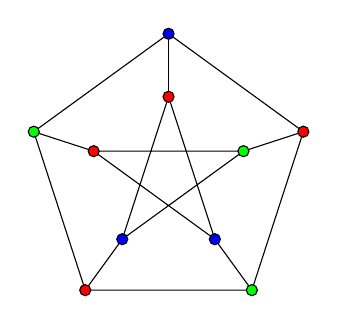
\begin{tikzpicture}
                \foreach \i in {1,...,5} {
                  \coordinate (a\i) at (72*\i + 18:1);
                  \coordinate (b\i) at (72*\i + 18:1.8);
                }

                \draw (a1) -- (a3) -- (a5) -- (a2) -- (a4) -- (a1);
                \draw (b1) -- (b2) -- (b3) -- (b4) -- (b5) -- (b1);
                \foreach \i in {1,...,5} {
                  \draw (a\i) -- (b\i);
                }
                \filldraw[fill=red] (a1) circle (2pt);
                \filldraw[fill=blue] (b1) circle (2pt);
                \filldraw[fill=red] (a2) circle (2pt);
                \filldraw[fill=green] (b2) circle (2pt);
                \filldraw[fill=blue] (a3) circle (2pt);
                \filldraw[fill=red] (b3) circle (2pt);
                \filldraw[fill=blue] (a4) circle (2pt);
                \filldraw[fill=green] (b4) circle (2pt);
                \filldraw[fill=green] (a5) circle (2pt);
                \filldraw[fill=red] (b5) circle (2pt);
              \end{tikzpicture}
        \end{figure}
        \textbf{Part 2:} $G$ is not planar. 
        \begin{proof}
            We label the vertices of $G$ as follows:
            \begin{figure}[H]
                \centering
                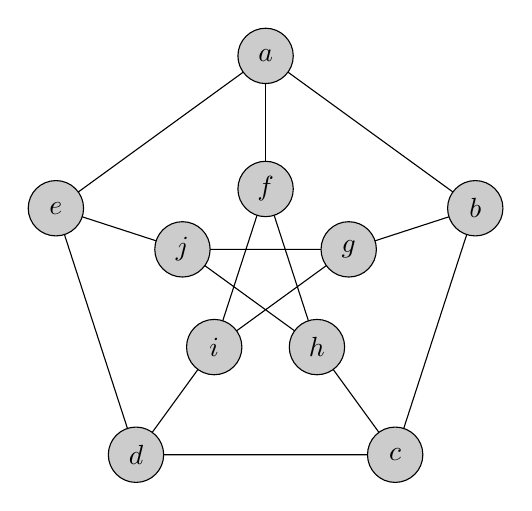
\begin{tikzpicture}
                    \foreach \i in {1,...,5} {
                      \coordinate (a\i) at (72*\i + 18:1.11);
                      \coordinate (b\i) at (72*\i + 18:2.8);
                    }

                    \draw (a1) -- (a3) -- (a5) -- (a2) -- (a4) -- (a1);
                    \draw (b1) -- (b2) -- (b3) -- (b4) -- (b5) -- (b1);
                    \foreach \i in {1,...,5} {
                      \draw (a\i) -- (b\i);
                    }
                    \node[vertex, fill=gray!40] at (a1) {$f$};
                    \node[vertex, fill=gray!40] at (a2) {$j$};
                    \node[vertex, fill=gray!40] at (a3) {$i$};
                    \node[vertex, fill=gray!40] at (a4) {$h$};
                    \node[vertex, fill=gray!40] at (a5) {$g$};
                    \node[vertex, fill=gray!40] at (b1) {$a$};
                    \node[vertex, fill=gray!40] at (b2) {$e$};
                    \node[vertex, fill=gray!40] at (b3) {$d$};
                    \node[vertex, fill=gray!40] at (b4) {$c$};
                    \node[vertex, fill=gray!40] at (b5) {$b$};
                  \end{tikzpicture}
            \end{figure}
            We will label the graph of $K_{3,3}$ as follows:
            \begin{figure}[H]
                \centering
                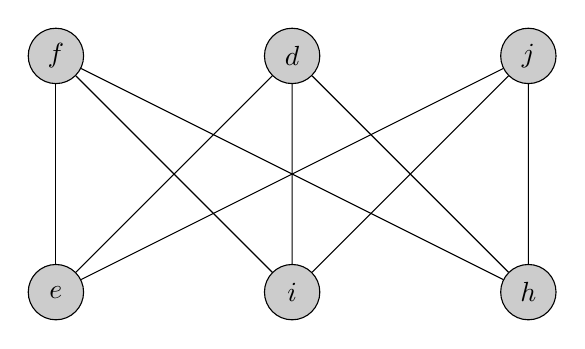
\begin{tikzpicture}[scale=1.5]
                    \node[vertex, fill=gray!40] (j) at (4,0) {$j$};
                    \node[vertex, fill=gray!40] (h) at (4,-2) {$h$};
                    \node[vertex, fill=gray!40] (i) at (2,-2) {$i$};
                    \node[vertex, fill=gray!40] (d) at (2,0) {$d$};
                    \node[vertex, fill=gray!40] (e) at (0,-2) {$e$};
                    \node[vertex, fill=gray!40] (f) at (0,0) {$f$};

                    \draw[edge, -] (j) -- (h);
                    \draw[edge, -] (j) -- (i);
                    \draw[edge, -] (j) -- (e);
                    \draw[edge, -] (d) -- (h);
                    \draw[edge, -] (d) -- (i);
                    \draw[edge, -] (d) -- (e);
                    \draw[edge, -] (f) -- (h);
                    \draw[edge, -] (f) -- (i);
                    \draw[edge, -] (f) -- (e); 
                \end{tikzpicture}
            \end{figure}
            We can create a graph $H$ that is homeomorphic to $K_{3,3}$ by a sequence of elementary subdivisions: 
            \begin{itemize}
                \item Removing the edge $\set*{d,h}$ and adding $\set*{d,c}$ and $\set*{c,h}$
                \item Removing the edge $\set*{e,f}$ and adding $\set*{e,a}$ and $\set*{a,f}$
                \item Removing the edge $\set*{i,j}$ and adding $\set*{i,g}$ and $\set*{g,j}$ 
            \end{itemize}
            $H$ is as follows:
            \begin{figure}[H]
                \centering
                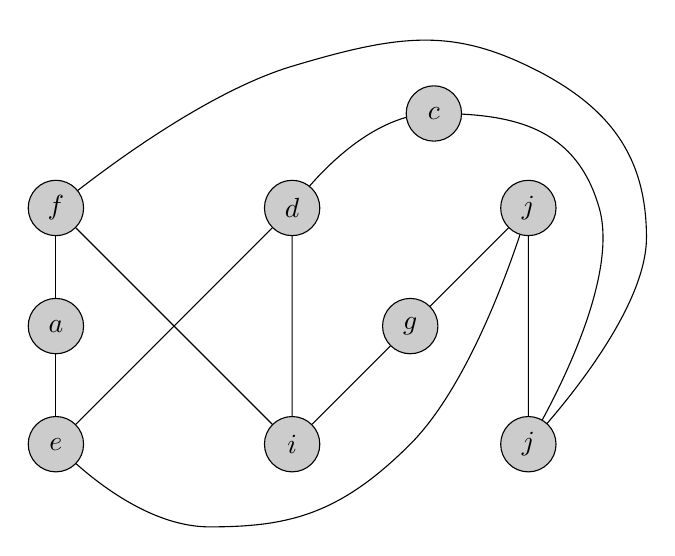
\begin{tikzpicture}[scale=1.5]
                    \begin{scope}[on above layer]
                        %%% Nodes
                        \node[vertex, fill=gray!40] (a) at (0,2) {$f$};
                        \node[vertex, fill=gray!40] (b) at (2,2) {$d$};
                        \node[vertex, fill=gray!40] (c) at (4,2) {$j$};
                        \node[vertex, fill=gray!40] (d) at (0,0) {$e$};
                        \node[vertex, fill=gray!40] (e) at (2,0) {$i$};
                        \node[vertex, fill=gray!40] (f) at (4,0) {$j$};
                        \node[vertex, fill=gray!40] (g) at (3.2,2.8) {$c$};
                        \node[vertex, fill=gray!40] (h) at (0,1) {$a$};
                        \node[vertex, fill=gray!40] (i) at (3,1) {$g$};
                    \end{scope}
        
                    %%% Edges
                    % \draw[edge] (a) to (d); Step 2
                    \draw[edge, -] (a) to (e);
                    \draw[edge, -] plot [smooth, tension=0.8] coordinates {(a) (2,3.2) (4,3.2) (5,1.75) (f)};
                    \draw[edge, -] (b) to (d);
                    \draw[edge, -] (b) to (e);
                    % \draw[edge] (b) to (f); Step 1
                    \draw[edge, -] plot [smooth, tension=0.8] coordinates {(c) (3,0) (1.3,-0.7) (d)};
                    \draw[edge, -] (c) to (e);
                    \draw[edge, -] (c) to (f);
        
                    %%% Step 1 Edges
                    \draw[edge, -] plot [smooth, tension=0.9] coordinates {(b) (g) (4.6,2) (f)};
        
                    %%% Step 2 Edges
                    \draw[edge, -] (a) to (h);
                    \draw[edge, -] (h) to (d);
                \end{tikzpicture}
            \end{figure}
            $H$ is isomorphic to the following graph:
            \begin{figure}[H]
                \centering
                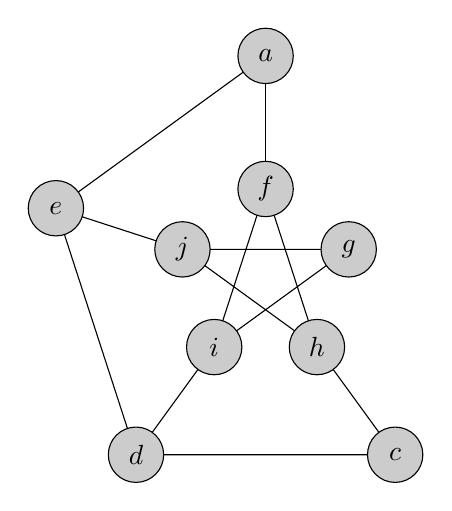
\begin{tikzpicture}
                    \foreach \i in {1,...,5} {
                      \coordinate (a\i) at (72*\i + 18:1.11);
                      \coordinate (b\i) at (72*\i + 18:2.8);
                    }

                    \draw (a1) -- (a3) -- (a5) -- (a2) -- (a4) -- (a1);
                    \draw (b1) -- (b2) -- (b3) -- (b4);
                    \foreach \i in {1,...,4} {
                      \draw (a\i) -- (b\i);
                    }
                    \node[vertex, fill=gray!40] at (a1) {$f$};
                    \node[vertex, fill=gray!40] at (a2) {$j$};
                    \node[vertex, fill=gray!40] at (a3) {$i$};
                    \node[vertex, fill=gray!40] at (a4) {$h$};
                    \node[vertex, fill=gray!40] at (a5) {$g$};
                    \node[vertex, fill=gray!40] at (b1) {$a$};
                    \node[vertex, fill=gray!40] at (b2) {$e$};
                    \node[vertex, fill=gray!40] at (b3) {$d$};
                    \node[vertex, fill=gray!40] at (b4) {$c$};
                  \end{tikzpicture}
            \end{figure}
            This graph is a subgraph of $G$, obtained by removing the vertex $b$ and its adjacent edges: $ba$, $bc$, and $bg$. As $H$ is a subgraph of $G$ and is homeomorphic to $K_{3,3}$, $G$ is not planar.
        \end{proof}
    \end{answer}
    % Question 12
    \begin{question}
        Prove that  Dijkstra's Algorithm  finds the length of the  shortest path between 2 vertices of a connected simple undirected  weighted  graph.\\ {\bf NOTE:} Check  the textbook.
    \end{question}

    % Answer 12
    \begin{answer}
        \begin{proof}
            By induction. Suppose there are two vertices $a$ and $z$. Let $P(n)$ be the statement that, at the $n$th iteration,
            \begin{enumerate}[\em i)]
                \item the label of every vertex $v$ in $S$ is the length of a shortest path from $a$ to this vertex, and
                \item the label of every vertex not in $S$ is the length of a shortest path from $a$ to this vertex that contains only (besides the vertex itself) vertices in $S$.
            \end{enumerate}
            \textbf{Base Case:} $n=0$. As there are no iterations that have been performed, $S = \emptyset$, so the length of a shortest path from $a$ to any vertex other than $a$ is $\infty$. Therefore, the basis is true.
            \\[12pt]
            \textbf{Inductive Hypothesis:} Suppose that $P(k)$ is true, $k \geq 1$. Let $v$ be the vertex added to $S$ at the $k+1$st iteration, meaning $v$ is the smallest label not a vertex in $S$ at the end of the $k$th iteration. We will show that $P(k) \to P(k+1)$.
            \\[12pt]
            \textbf{Inductive Step:} From the inductive hypothesis, the vertices in $S$ prior to the $k+1$st iteration have the shortest path from $a$ to them and $v$ is labeled with the length of the shortest path from $a$ to $v$. We will prove this by contradiction. 
            \\[12pt]
            If this was not true, then there exists a shorter path from $a$ to $v$ containing at least one vertex not in $S$. Let $u$ be the first of these vertices not in $S$ in the path from $a$ to $v$. From the inductive hypothesis \textit{(ii)}, the path from $a$ to $u$ is shorter than the path from $a$ to $v$. Therefore, the path from $a$ to $v$ is not the shortest path from $a$ to $v$. $\contradiction$
            \\[12pt]
            This contradicts the choice of $v$. Thus, \textit{(i)} holds for the $k+1$st iteration.
            \\[12pt]
            Let $u$ be a vertex not in $S$ after $k+1$ iterations. If the shortest path from $a$ to $u$ does not contain $v$, then, by the inductive hypothesis, its length, $L_k(u)$. If it does contain $v$, then the path is made up of a path from $a$ to $v$ of shortest possible length using elements in $S$ other than $v$, followed by the edge from $v$ to $u$. In this case, its length is $L_k(v) + w(u,v)$. Therefore, \textit{(ii)} is true because $L_{k+1}(u)$ minimizes $L_k(u)$, producing the least value for $L_{k+1}(u)$.
            \\[12pt]
            Thus, $P(k+1)$ is true. Therefore, $P(n)$ is true for all $n \geq 0$. Therefore, Dijkstra's Algorithm finds the length of the shortest path between 2 vertices of a connected simple undirected weighted graph.
        \end{proof}
    \end{answer}
\end{document} 
